\def\lo#1{ -- ++(#1,0) }
\def\hi#1{ |- ++(#1,1) -- ++(0,-1) }
\def\hop#1#2{\lo{#1}\hi{#2}}

\def\periodend#1#2#3{
   \begin{scope}
     \clip  (#1 + 0.2, #2 - 0.2) rectangle (#1, #2 + 0.2);
     \draw[#3] (#1, #2) circle (3pt);
   \end{scope}
}
\def\periodbegin#1#2#3{
   \begin{scope}
     \clip  (#1 + 0.2, #2 - 0.2) rectangle (#1, #2 + 0.2);
     \fill[#3] (#1, #2) circle (3pt);
   \end{scope}
}
\def\period#1#2#3{
   \clip (#1, #2) circle (3pt);
}


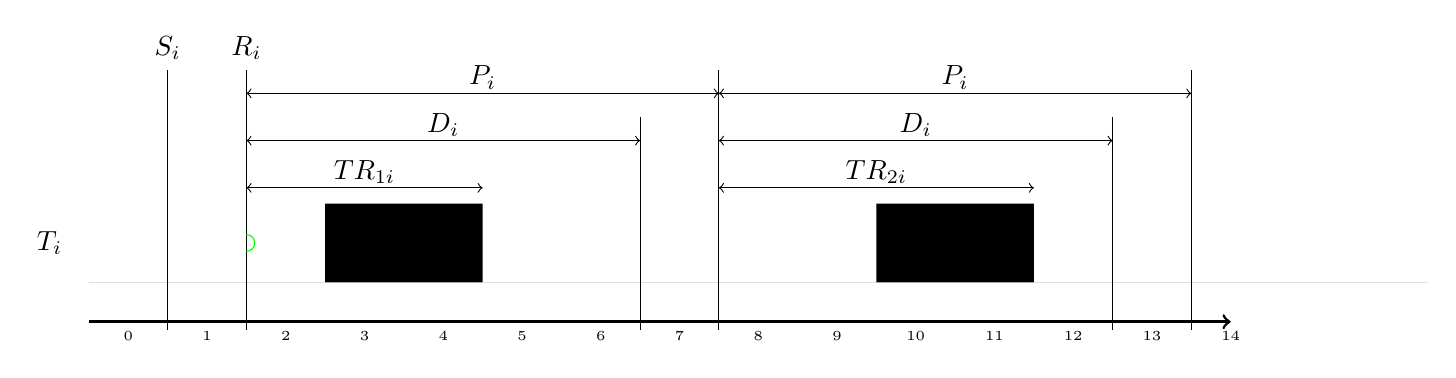
\begin{tikzpicture}[scale=1]
   %\draw[xstep=1,ystep=0.1,gray,very thin] (0,0) grid (#1.5,#2);
   \draw[->, line width=1pt] (0,-2) -- (14.5,-2) coordinate (x axis);
   %\draw[line width=1pt] (0,#2) -- (0,0) coordinate (x axis);
   \foreach \x in {0,1,...,14}
      \draw (\x.5,-2) node[anchor=north] {\tiny\x};
   %\foreach \i in {2, 8, 14}
    %\draw  (\i, -1) circle (3pt);
   \fill  (0,-1.5) \lo 3 \hi 2 \lo 5 \hi 2 \lo 5;
   \draw (-0.5,-1) node {$T_i$};
   \draw (1,-2.1) -- (1,1.2) node[above] {$S_i$};
   \draw (2,-2.1) -- (2,1.2) node[above] {$R_i$};
   \draw (7,-2.1) -- (7,0.6);
   \draw (8,-2.1) -- (8,1.2);
   \draw (13,-2.1) -- (13,0.6);
   \draw (14,-2.1) -- (14,1.2);
   \draw[<->] (2,-.3) -- (5,-.3) node[above=-2,pos=0.5] {$TR_{1i}$};
   \draw[<->] (2,0.3) -- (7,0.3) node[above=-2,pos=0.5] {$D_i$};
   \draw[<->] (2,0.9) -- (8,0.9) node[above=-2,pos=0.5] {$P_i$}; 
   \draw[<->] (8,-0.3) -- (12,-0.3) node[above=-2,pos=0.5] {$TR_{2i}$};
   \draw[<->] (8,0.3) -- (13,0.3) node[above=-2,pos=0.5] {$D_i$};
   \draw[<->] (8,0.9) -- (14,0.9) node[above=-2,pos=0.5] {$P_i$};
   \periodend{2}{-1}{green}
%   \begin{scope}
 %    \clip  (2.2, -0.8) rectangle (2.0, -1.2);
  %   \draw  (2, -1) circle (3pt);
   %\end{scope}

\end{tikzpicture}